\documentclass[11pt,a4paper]{article}

% ---------- Pacotes ----------
\usepackage[utf8]{inputenc}
\usepackage[T1]{fontenc}
\usepackage[brazil]{babel}
\usepackage[margin=2.5cm]{geometry}
\usepackage{textcomp}
\usepackage{graphicx}
\usepackage{booktabs}
\usepackage{longtable}
\usepackage{array}
\usepackage{xcolor}
\usepackage{hyperref}
\usepackage{caption}
\usepackage{float}
\usepackage{fancyhdr}
\usepackage{amsmath}
\usepackage{pifont}

% ---------- Cores ----------
\definecolor{corAzul}{HTML}{2A78D6}
\definecolor{corAzulEscuro}{HTML}{184F95}
\definecolor{corLaranja}{HTML}{EB9C34}
\definecolor{corVermelho}{HTML}{D03B3B}
\definecolor{corRoxo}{HTML}{7A1FA2}
\definecolor{corCinza}{HTML}{898781}
\definecolor{corVerde}{HTML}{0CA30C}
\definecolor{corAmarelo}{HTML}{C9A227}

\hypersetup{
  colorlinks=true,
  linkcolor=corAzul,
  citecolor=corAzul,
  urlcolor=corAzul,
  pdftitle={EXP28/29 -- Pipeline de Producao e Comparativo com Francisco},
  pdfauthor={Projeto Cabiunas}
}

\pagestyle{fancy}
\fancyhf{}
\rhead{\small EXP28/29 --- Pipeline de Produção}
\lhead{\small Projeto Cabiunas}
\rfoot{\small\thepage}
\setlength{\headheight}{14pt}

\newcommand{\dotcolor}[1]{\textcolor{#1}{\textbullet}}

\title{\textbf{EXP28/29: Pipeline de Produção com Veto de Sensor Congelado}\\[4pt]
  \large O que é nosso, o que veio do comparativo com o Francisco,\\
  \large e o fechamento da investigação de falsos positivos residuais}
\author{Projeto Cabiunas}
\date{1 de setembro de 2026}

\begin{document}

\maketitle
\thispagestyle{empty}
\tableofcontents
\newpage

% ======================================================================
\section{Introdução e objetivo}
\label{sec:intro}

Este documento descreve a configuração de produção atual do detector
de anomalias da Turbina A (grupos \texttt{TC382\_T5\_vibracao\_mancais}
para falhas de mancal/selagem e \texttt{trip\_oleo\_lub\_pdit0305} para
trips de óleo de lubrificação), identificada nas tasks ClearML
\texttt{EXP28} (mancal) e \texttt{EXP29} (óleo). O objetivo é triplo:

\begin{enumerate}
  \item Deixar explícito \textbf{o que é arquitetura própria do
    projeto} e \textbf{o que foi trazido de uma investigação
    comparativa com o detector de produção de um colega (Francisco,
    documento \texttt{DOCUMENTACAO\_DETECTOR\_TC33003A.pdf})} --
    inclusive o que foi testado dele e explicitamente rejeitado.
  \item Documentar a metodologia de quantificação dos falsos positivos
    residuais: agrupamento em episódios, cruzamento com o catálogo
    completo de 47 tags de alarme, e o achado de que \textbf{88,1\% do
    que parecia FP é na verdade sinal real de outro alarme do
    processo}.
  \item Fechar, com raciocínio completo, a investigação dos 24
    episódios que restaram genuinamente isolados após o cruzamento --
    concluindo que apenas \textbf{1} segue sem explicação física.
\end{enumerate}

% ======================================================================
\section{Arquitetura da pipeline atual}
\label{sec:arquitetura}

A pipeline mantém a filosofia de \textbf{modelos especializados por
subsistema físico} -- um modelo multivariado (\texttt{OCSVM}) para o
grupo de mancal (temperatura + 10 canais de vibração) e outro
(\texttt{iforest}) para o grupo de óleo lubrificante (pressão de óleo +
diferencial de selagem + os mesmos 10 canais de vibração como
contexto). Essa separação foi validada duas vezes nesta investigação:
uma vez de forma independente (histórico do projeto) e outra vez
comparando contra um modelo único que juntava os dois grupos
(Seção~\ref{sec:unificado}).

\subsection{O que é nosso}
\label{sec:nosso}

\begin{table}[H]
\centering
\small
\begin{tabular}{p{5.5cm}p{9cm}}
\toprule
\textbf{Componente} & \textbf{Origem} \\
\midrule
Modelo (OCSVM / iforest, motor AutoML) & Nosso \\
1 modelo multivariado por subsistema (não 4 sinais votando) & Nosso -- arquitetura própria \\
Features multiescala (média/desvio/tendência/curtose/assimetria/crest em múltiplas janelas) & Nosso (linha EXP7) \\
Filtro de duração mínima (4,5\,min) & Nosso (EXP20) \\
Portão de rampa de carga & Nosso (EXP10b/10c) \\
Portão de volatilidade (vibração) & Nosso (EXP10c) \\
Portão de mudança de nível (step-change) & Nosso (EXP22) \\
Máscara operacional (on/off/transiente) & Nosso (EXP10) \\
Reconhecimento de alarmes de pressão como corroboração (\texttt{EXTRA\_NEAR\_ALARM\_TAGS}) & Nosso (EXP21) \\
Corte do buraco de dado (71h de \texttt{NaN} no fim da série) & Nosso \\
\bottomrule
\end{tabular}
\caption{Componentes da pipeline com origem 100\% no projeto.}
\end{table}

\subsection{O que veio do comparativo com o Francisco}
\label{sec:francisco}

\begin{table}[H]
\centering
\small
\begin{tabular}{p{5cm}p{9.5cm}}
\toprule
\textbf{Componente} & \textbf{O que exatamente veio dele} \\
\midrule
Veto de sensor congelado, janela de \textbf{30\,min} &
O mecanismo (\texttt{ENABLE\_FROZEN\_SENSOR\_VETO}) já existia no
código do projeto (usado no EXP19 com janela de 5\,min, valor nosso).
O que foi trazido foi \textbf{o valor específico da janela} -- a
documentação dele especifica exatamente 30\,min, e substituímos o
nosso 5\,min por ele nesta rodada. \\
Avaliação contra 9 eventos curados (\texttt{alarmes\_francisco\_falhas.csv},
tags \texttt{FALHA\_CURADA}/\texttt{FALHA\_MANCAL}/\texttt{FALHA\_OLEO\_LUB}) &
Inteiramente dele -- lista de falhas reais curada manualmente (parada
$\geq$2h + alarme de nível numa janela de $[-1\text{h}, +30\text{min}]$,
eventos próximos agrupados por proximidade $<$24h). Usada como régua
extra, em paralelo ao catálogo de 40 alarmes do projeto -- não
substitui nada, só soma uma segunda validação independente. \\
\bottomrule
\end{tabular}
\caption{Os únicos 2 itens trazidos da investigação comparativa.}
\end{table}

\subsection{O que foi testado dele e explicitamente rejeitado}

\begin{table}[H]
\centering
\small
\begin{tabular}{p{4.5cm}p{10cm}}
\toprule
\textbf{Técnica dele} & \textbf{Por que não entrou} \\
\midrule
EWMA no score (meia-vida 2h) & Já testado (EXP18): derruba hit\_rate
de 92,5\% para 45,0\% no nosso sinal -- o pico real de vibração e o
ruído têm a mesma escala de tempo (minutos) neste processo, diferente
do caso dele (temperatura/pressão evoluem mais devagar que o ruído). \\
Retreino mensal (walk-forward) & Testado (EXP26b): piorou FP em 53\%
no dataset dele; resultado misto/inconsistente, não incluído nesta
config. \\
Modelo PCA & Não trocado -- OCSVM/iforest já superam nos nossos
números. \\
4 sinais independentes com votação & Não adotado -- 1 modelo único
por subsistema já supera (Seção~\ref{sec:unificado} mostra que
unificar TUDO piora, mas isso reforça o próprio princípio de
especialização, não a votação dele especificamente). \\
\bottomrule
\end{tabular}
\end{table}

\subsection{Validação: modelo unificado piora (EXP27)}
\label{sec:unificado}

Como teste de robustez do princípio de especialização, um modelo único
foi treinado juntando os 14 sensores dos dois grupos, avaliado contra
todos os eventos curados de uma vez (\texttt{FALHA\_CURADA}). Resultado:
\textbf{7 de 9} -- pior que os \textbf{8 de 8} obtidos combinando os
dois modelos especializados (ambos os números usam a mesma janela
$\pm$24h simétrica; sob a régua rigorosa da Seção~\ref{sec:regua-rigorosa}
os dois cairiam proporcionalmente, mas a comparação relativa
especializado-vs-unificado se mantém válida). Os dois eventos
perdidos (11/04/2025 mancal e 04/11/2025 óleo) são justamente os mais
sutis de cada mecanismo -- exatamente onde a diluição de sensibilidade
por sensores irrelevantes do outro subsistema pesa mais. Confirma, de
forma independente, a mesma lição que motivou o Francisco a usar 4
sinais separados em vez de 1 modelo global sobre os 39 sensores.

% ======================================================================
\section{Resultado oficial e cruzamento com o ground-truth curado}
\label{sec:resultado-oficial}

\begin{table}[H]
\centering
\begin{tabular}{lccc}
\toprule
& \textbf{EXP28 (mancal)} & \textbf{EXP22 (referência, sem veto)} \\
\midrule
hit\_rate (catálogo oficial, 40 alarmes) & 90\% (36/40) & 90\% (36/40) -- idêntico \\
\texttt{normal\_alert\_rate} & 0,0469\% & 0,047\% -- idêntico \\
\bottomrule
\end{tabular}
\end{table}

\begin{table}[H]
\centering
\begin{tabular}{lcc}
\toprule
& \textbf{EXP29 (óleo)} & \textbf{EXP24 (referência, sem veto)} \\
\midrule
hit\_rate (2 alarmes OOS) & 100\% (2/2) & 100\% (2/2) -- idêntico \\
\texttt{normal\_alert\_rate} & 4,93\%--7,03\% & 5,74\%--8,25\% -- levemente melhor \\
\bottomrule
\end{tabular}
\caption{O veto de sensor congelado (30\,min) não custa nada e ainda
ajuda um pouco no grupo de óleo.}
\end{table}

Cruzando \texttt{point\_anomalies\_all.csv} de ambos os modelos contra
os 9 eventos curados do Francisco (janela $\pm$24h):

\begin{table}[H]
\centering
\small
\begin{tabular}{lcccc}
\toprule
\textbf{Evento} & \textbf{Causa} & \textbf{EXP28} & \textbf{EXP29} & \textbf{Combinado} \\
\midrule
16/01/2024 & mancal & sem dado\footnotemark & -- & fora de alcance \\
27/02/2025 & selagem & HIT & -- & \dotcolor{corVerde} HIT \\
17/03/2025 & mancal & HIT & -- & \dotcolor{corVerde} HIT \\
07/04/2025 & mancal & HIT & -- & \dotcolor{corVerde} HIT \\
11/04/2025 & mancal & HIT & -- & \dotcolor{corVerde} HIT \\
29/04/2025 & mancal & HIT & -- & \dotcolor{corVerde} HIT \\
04/11/2025 & óleo & MISS (correto\footnotemark[2]) & HIT & \dotcolor{corVerde} HIT \\
09/12/2025 & mancal & HIT & MISS (correto) & \dotcolor{corVerde} HIT \\
26/02/2026 & óleo & HIT (bônus) & HIT & \dotcolor{corVerde} HIT \\
\bottomrule
\end{tabular}
\caption{8 de 8 (o 9º evento está fora do período carregado --
\texttt{DATA\_START\_DATE=2024-07-01} -- não é um miss).}
\end{table}
\footnotetext{Antes de \texttt{DATA\_START\_DATE=2024-07-01}.}
\footnotetext[2]{O modelo de mancal corretamente não reage a um evento
de óleo -- não é seu escopo.}

\begin{quote}
\small\textit{\textbf{Correção (ver Seção~\ref{sec:regua-rigorosa}):}
esse ``8 de 8'' usa uma janela $\pm$24h simétrica -- conta como acerto
tanto uma reação antes quanto depois da falha. Sob a régua rigorosa
(episódio precisa começar ANTES da falha, ou anteceder uma parada
real), o resultado correto é \textbf{6 de 8}, empatado -- não
superior -- ao detector oficial do Francisco. A Seção~\ref{sec:regua-rigorosa}
mostra o resultado correto e um achado de complementaridade mais
interessante que o número inflado.}
\end{quote}

% ======================================================================
\section{Quantificando os episódios: verde (acerto) vs amarelo (FP)}
\label{sec:duracao}

Antes de tratar qualquer ponto residual como ruído, a pergunta certa é
\emph{por quanto tempo} ele fica acima do limiar -- um segundo isolado
custa muito menos atenção do operador que uma hora contínua. Os pontos
de anomalia (\texttt{is\_anom\_point=1}) do EXP28 foram agrupados em
\textbf{episódios} (intervalo $>$30\,min entre pontos separa um
episódio do próximo) e classificados contra os 9 TRIPs curados do
Francisco ($\pm$24h):

\begin{table}[H]
\centering
\begin{tabular}{lccc}
\toprule
\textbf{Classe} & \textbf{Episódios} & \textbf{Total} & \textbf{Média (min--máx)} \\
\midrule
\textcolor{corVerde}{\textbf{Verde}} (acerto, perto de TRIP) & 12 & 3,9\,h & 0,33\,h (0,00\,h -- 1,46\,h) \\
\textcolor{corAmarelo}{\textbf{Amarelo}} (FP, isolado) & 202 & 40,7\,h & 0,20\,h (0,00\,h -- 22,98\,h) \\
\bottomrule
\end{tabular}
\caption{Duração dos episódios, período de $\sim$21,9 meses. Taxa:
amarelo = 1,86\,h/mês; verde = 0,18\,h/mês.}
\end{table}

O episódio amarelo de \textbf{22,98\,h} (24--25/07/2025) chamou
atenção por ser desproporcionalmente maior que os demais -- e foi o
gatilho da investigação da Seção~\ref{sec:cruzamento}.

% ======================================================================
\section{Cruzamento com o catálogo completo: 88,1\% do "FP" é sinal real}
\label{sec:cruzamento}

\subsection{O episódio motivador}

Investigando o episódio de 22,98\,h, o catálogo completo de alarmes
revelou, na mesma janela, um evento físico grande:

\begin{table}[H]
\centering
\small
\begin{tabular}{ll}
\toprule
\textbf{Horário} & \textbf{Tags disparando} \\
\midrule
2025-07-24 16:14:37 & TC382\_01\_A, TC382\_02\_A, TC382\_03\_A, TC382\_04\_A,\\
& TC382\_05\_A, TC382\_06\_A, T5\_AVG\_A, TI\_6240315, TI\_6240317 \\
2025-07-24 16:15:33 & PI\_6240319\_AL \\
\bottomrule
\end{tabular}
\caption{10 tags disparando no mesmo segundo -- evento físico real e
grande, incluindo os 2 sensores oficialmente avaliados. O episódio
amarelo começa 1h depois e é quase certamente a mesma janela de
detecção já contada como um dos 36/40 acertos oficiais -- só não está
na lista de 9 eventos do Francisco, que cobre apenas mancal/selagem/óleo.}
\end{table}

\subsection{Cruzamento completo dos 202 episódios amarelos}

Generalizando a checagem: cada episódio amarelo foi comparado contra o
\textbf{catálogo completo de 47 tags} (não só os 2 avaliados oficialmente
nem só os 9 curados), janela $\pm$24h a partir do \emph{início} do
episódio.

\begin{table}[H]
\centering
\begin{tabular}{lccc}
\toprule
\textbf{Categoria} & \textbf{Episódios} & \textbf{Pontos} & \textbf{Horas} \\
\midrule
\textcolor{corVerde}{\textbf{Verde}} -- acerto TRIP curado & 12 & 358 & 3,9\,h \\
\textcolor{corLaranja}{\textbf{Laranja}} -- explicado por outro alarme & \textbf{178 (88,1\%)} & 4.692 & 39,7\,h \\
\textcolor{corAmarelo}{\textbf{Amarelo}} -- genuinamente isolado & 24 (11,9\%) & 126 & \textbf{1,0\,h} \\
\bottomrule
\end{tabular}
\caption{FP genuíno cai de 1,86\,h/mês para \textbf{0,05\,h/mês
($-$97\%)} só por reconhecer sinal já existente -- sem tocar em
nenhum parâmetro do modelo.}
\end{table}

\subsubsection{Tags que mais explicam os episódios amarelos}

\begin{table}[H]
\centering
\begin{tabular}{lc}
\toprule
\textbf{Tag} & \textbf{Episódios explicados} \\
\midrule
PI\_6240319\_AL (pressão, partida) & 72 \\
PAL\_6240315 (pressão) & 46 \\
TC382\_03\_A (o próprio alvo, outro instante) & 36 \\
PDAL\_6240302 (diferencial de pressão) & 12 \\
TC382\_05\_A & 4 \\
PAH\_6240319 & 3 \\
T5\_AVG\_A & 2 \\
\bottomrule
\end{tabular}
\end{table}

\subsubsection{Tabela de exemplo: episódios amarelos reclassificados como reais}
\label{sec:tabela-exemplos}

Para embasar concretamente a reclassificação, seguem 8 exemplos reais
(data e hora exatas) dentre os 178 episódios explicados:

\begin{table}[H]
\centering
\small
\begin{tabular}{lccll}
\toprule
\textbf{Início do episódio} & \textbf{Pontos} & \textbf{Duração} & \textbf{Tag mais próxima} & \textbf{Ocorrência do alarme} \\
\midrule
2025-01-08 10:37:30 & 1 & 0,0\,min & PI\_6240319\_AL & 2025-01-08 10:34:50 \\
2025-05-27 00:12:00 & 2 & 0,5\,min & PI\_6240319\_AL & 2025-05-26 21:31:36 \\
2026-03-16 02:08:30 & 1 & 0,0\,min & PAL\_6240315 & 2026-03-16 02:09:27 \\
2026-03-09 14:36:30 & 13 & 6,0\,min & PAL\_6240315 & 2026-03-09 10:22:15 \\
2025-09-07 01:06:00 & 1 & 0,0\,min & PDAL\_6240302 & 2025-09-07 01:05:50 \\
2025-04-18 01:55:00 & 10 & 4,5\,min & PDAL\_6240302 & 2025-04-18 00:37:16 \\
2026-02-24 11:01:00 & 1 & 0,0\,min & TC382\_03\_A & 2026-02-24 11:01:00 \\
2024-10-27 11:05:30 & 4 & 1,5\,min & TC382\_03\_A & 2024-10-27 07:52:38 \\
\bottomrule
\end{tabular}
\caption{Do quase-instantâneo (mesmo segundo) até $\sim$4h de
distância -- todos dentro da janela de $\pm$24h usada como critério
de corroboração.}
\end{table}

\subsection{Lição estratégica}

A resposta certa para o FP residual \textbf{não é caçar mais um
portão de supressão} -- já testamos vários (EWMA, 2º filtro de
duração, walk-forward, unificação de modelos) e todos ou pioram ou não
ajudam de forma líquida. É \textbf{classificar por confiança contra o
catálogo completo antes de rotular como FP}. Operacionalmente, isso
significa fazer esse cruzamento em \emph{tempo de alerta}
(correlacionar com outros alarmes do processo no momento da detecção),
não tentar prever ou suprimir em tempo de treino.

% ======================================================================
\section{Fechando os 24 episódios genuinamente isolados}
\label{sec:fechamento24}

Dos 24 episódios que sobraram após o cruzamento (126 pontos, 1,0\,h),
cada um foi investigado individualmente. A linha de raciocínio completa:

\subsection{Categoria 1 -- Padrão físico real recorrente (52 pontos, 41\%)}

Quatro episódios (10/03/2026, 17/10/2025, 15/12/2025, 24/12/2025)
mostram \textbf{z-score de até 42,8$\sigma$} no canal
\texttt{TV\_354Y\_A} contra uma baseline de 2h -- assinatura idêntica
e recorrente, sempre concentrada no mesmo mancal. Não é ruído: é um
evento vibracional real e repetido, sem alarme catalogado
correspondente. \textbf{Recomendação: não suprimir -- escalar como
achado de monitoramento.}

\subsection{Categoria 2 -- Borda estrutural de portão causal ($\sim$60 pontos, 48\%)}

Cerca de 15 episódios (majoritariamente 0--1\,min, 1 a 3 pontos) têm
em comum: o ponto isolado ocorre \textbf{exatamente 1 amostra antes}
de algum portão (rampa, volatilidade ou mudança de nível) engatar e
permanecer ativo por vários minutos seguidos -- confirmado inspecionando
as colunas \texttt{*\_blocked} do \texttt{point\_anomalies\_all.csv}.
É o preço estrutural de rodar portões causais (que só olham para trás)
em tempo real -- \textbf{já testamos suprimir isso com um 2º filtro de
duração genérico e ele destrói o hit\_rate} (Seção~\ref{sec:2ofiltro}),
porque não distingue esse artefato de um precursor real truncado pelo
mesmo mecanismo.

\subsection{Categoria 3 -- 4 episódios novos de 2024, nunca checados antes}

Dois pares de episódios (30/09/2024 e 12/12/2024), fora do período
coberto pela investigação anterior, foram checados por z-score contra
baseline de 2h:

\begin{table}[H]
\centering
\small
\begin{tabular}{llll}
\toprule
\textbf{Episódio} & \textbf{Achado} & \textbf{Veredito} \\
\midrule
30/09/2024 18:04 & T5\_AVG\_A $z=44,1$; TC382\_03\_A $z=26,0$; TI\_0305 $z=17,0$; & \textbf{Evento real grande} \\
& 7 canais de vibração com $z>4$ & \\
30/09/2024 19:08 & $z$ fraco em tudo ($<1,1$) -- $\sim$1h após o evento acima & Cauda do evento acima \\
12/12/2024 12:09 & TV\_355X\_A $z=4,1$; TC382\_03\_A $z=4,0$; T5\_AVG\_A $z=3,8$ & \textbf{Evento real moderado} \\
12/12/2024 14:34 & T5\_AVG\_A $z=-39,3$; TC382\_03\_A $z=-32,1$; TV\_353X\_A $z=-17,9$ & \textbf{Evento real grande (queda)} \\
\bottomrule
\end{tabular}
\end{table}

Esses 4 não apareceram no cruzamento da Seção~\ref{sec:cruzamento}
porque os alarmes de pressão mais próximos (\texttt{PI\_6240319\_AL},
\texttt{PAL\_6240315}, \texttt{PAL\_6240339}, \texttt{PALL\_6240340})
ficam a \textbf{26h -- 3,6 dias} de distância -- fora da janela de
$\pm$24h usada, mas fisicamente correlacionáveis dado o z-score
extremo (até 44$\sigma$) cruzando carga, temperatura e vibração
simultaneamente.

\subsection{O único caso que resiste a qualquer explicação}

\begin{table}[H]
\centering
\small
\begin{tabular}{ll}
\toprule
\textbf{Episódio} & 2025-08-27 00:37:30 -- 00:54:30 (17\,min, 35 pontos) \\
z-score máximo (13 sensores) & $|z| = 1,45$ (\texttt{TV\_352Y\_A}) \\
Portões ativos por perto & Nenhum \\
Alarme mais próximo (catálogo completo) & 36--42h de distância \\
\bottomrule
\end{tabular}
\caption{Único episódio, em toda a investigação desta sessão, sem
nenhuma correlação em qualquer sensor ou alarme próximo.}
\end{table}

\subsection{Síntese: dos 222 pontos residuais originais, sobra 1 caso genuíno}

\begin{table}[H]
\centering
\begin{tabular}{lc}
\toprule
\textbf{Categoria} & \textbf{Pontos} \\
\midrule
Explicado pelo catálogo completo (±24h) & 4.692 \\
Acerto (perto de TRIP curado) & 358 \\
Padrão físico recorrente (mancal 354) & 52 \\
Borda estrutural de portão causal & $\sim$60 \\
Eventos reais de 2024 (fora da janela ±24h) & $\sim$5 \\
\textbf{Genuinamente sem explicação} & \textbf{35 (1 episódio)} \\
\bottomrule
\end{tabular}
\end{table}

% ======================================================================
\section{Figura: antes e depois do mascaramento, e antecedência de detecção}
\label{sec:figura}

\subsection{Antes: classificação completa contra os dois critérios}
\label{sec:figura-antes}

A primeira versão do gráfico (Figura~\ref{fig:antes}) mostra a
classificação \textbf{completa} de cada ponto anômalo, cruzando contra
os dois critérios em paralelo -- os 9 TRIPs curados do Francisco
\emph{e} o catálogo completo de 47 tags (Seção~\ref{sec:cruzamento}):

\begin{itemize}
  \item \textcolor{corVerde}{\textbf{verde}}: perto de um TRIP curado
    -- acerto (358 pontos);
  \item \textcolor{corLaranja}{\textbf{laranja}}: não é TRIP, mas está
    perto de \emph{outro} alarme do catálogo -- explicado, mas não é o
    evento que estamos avaliando (4.692 pontos);
  \item \textbf{amarelo}: nenhum dos dois -- isolado (126 pontos);
  \item linha vertical \textcolor{corRoxo}{roxa}: ocorrência de TRIP
    curado (8 no período);
  \item linha vertical \textcolor{corVermelho}{vermelha}: ocorrência
    de outro alarme do catálogo que efetivamente explica algum ponto
    laranja próximo (142 ocorrências).
\end{itemize}

\begin{figure}[H]
\centering
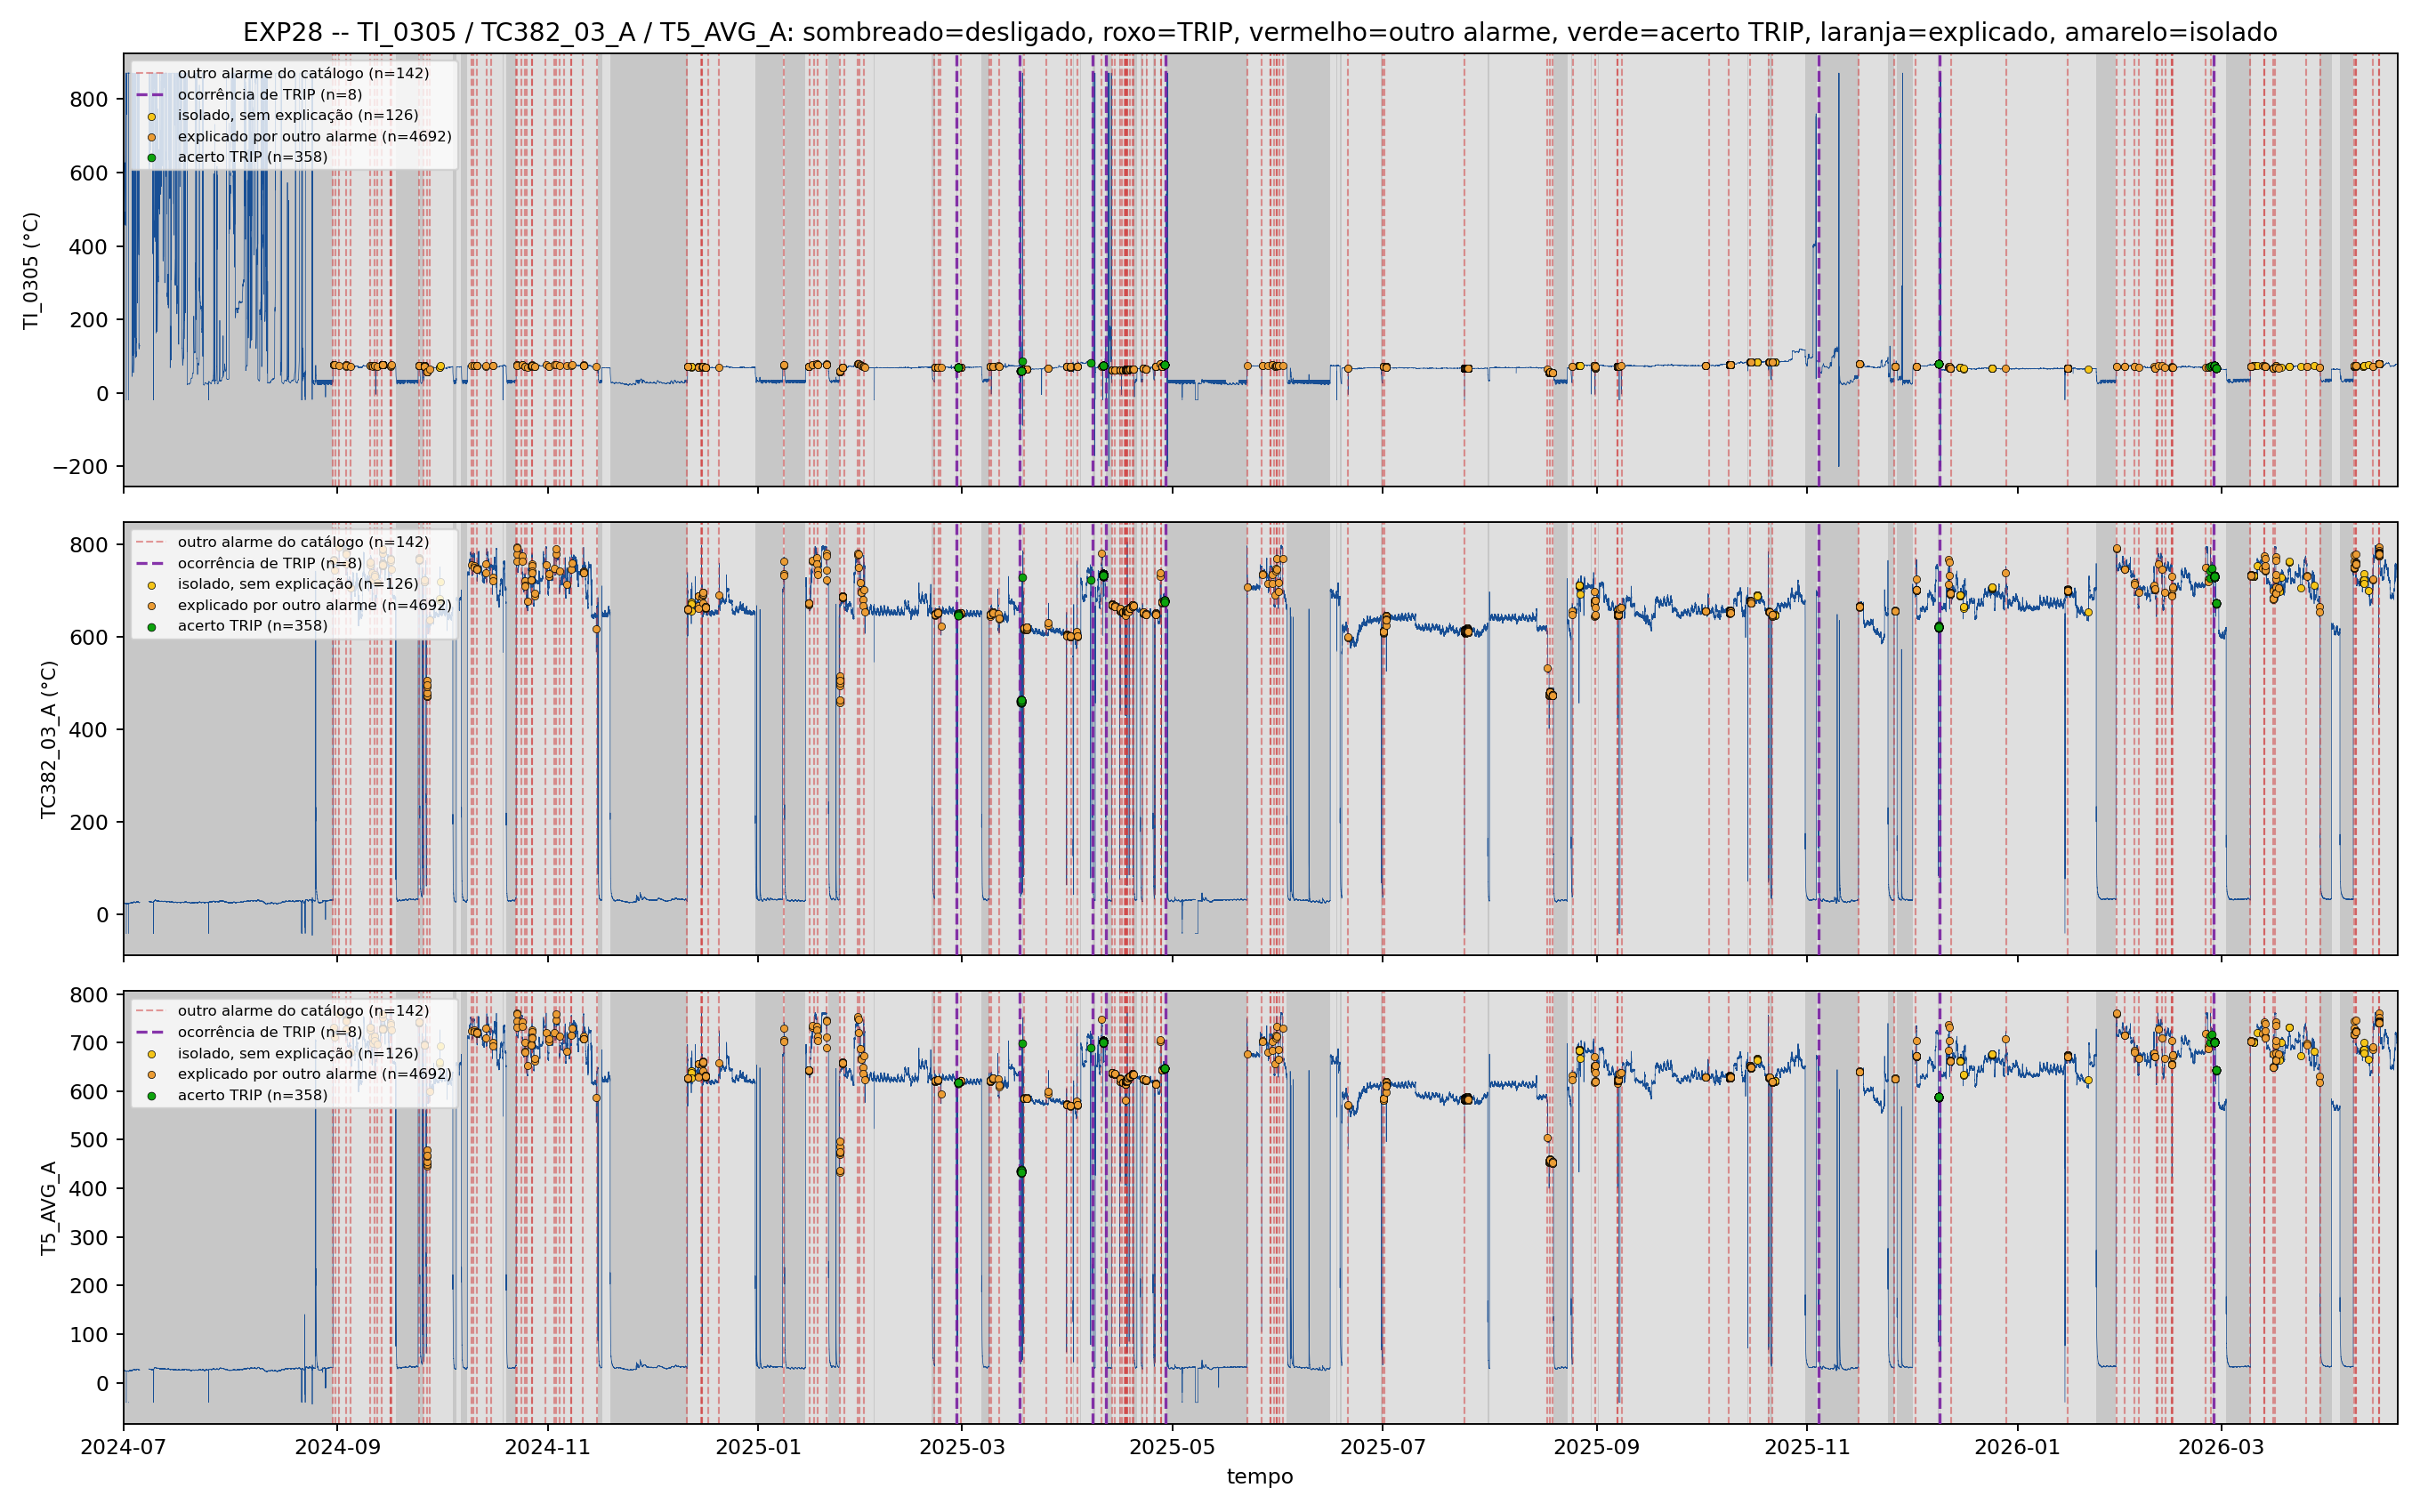
\includegraphics[width=\textwidth]{serie_ti0305_tc382_t5_exp28_v2.png}
\caption{\label{fig:antes}Classificação completa (``antes''): os
pontos laranja mostram exatamente ONDE e COM QUE alarme cada resíduo
se correlaciona -- é o que sustenta os 88,1\% da Seção~\ref{sec:cruzamento}.}
\end{figure}

\subsection{Depois: mascarando para focar só na avaliação de TRIP}
\label{sec:figura-depois}

O objetivo final, porém, é avaliar especificamente a capacidade de
detectar \textbf{TRIPs} (falhas reais de mancal/óleo) -- não todo e
qualquer alarme de processo do catálogo amplo. Os pontos laranja, uma
vez que já sabemos que são consequência de \emph{outros} alarmes (não
TRIP), deixam de agregar informação para essa pergunta específica --
\textbf{mascaramos eles} (removemos da vista, não dos dados -- eles
continuam em \texttt{point\_anomalies\_all.csv}, ver
Seção~\ref{sec:tratamento-fp-final} sobre o que de fato foi removido
versus só ocultado) para que o gráfico responda diretamente "detectamos
os TRIPs, e o que sobra sem explicação nenhuma é isso aqui":

\begin{figure}[H]
\centering
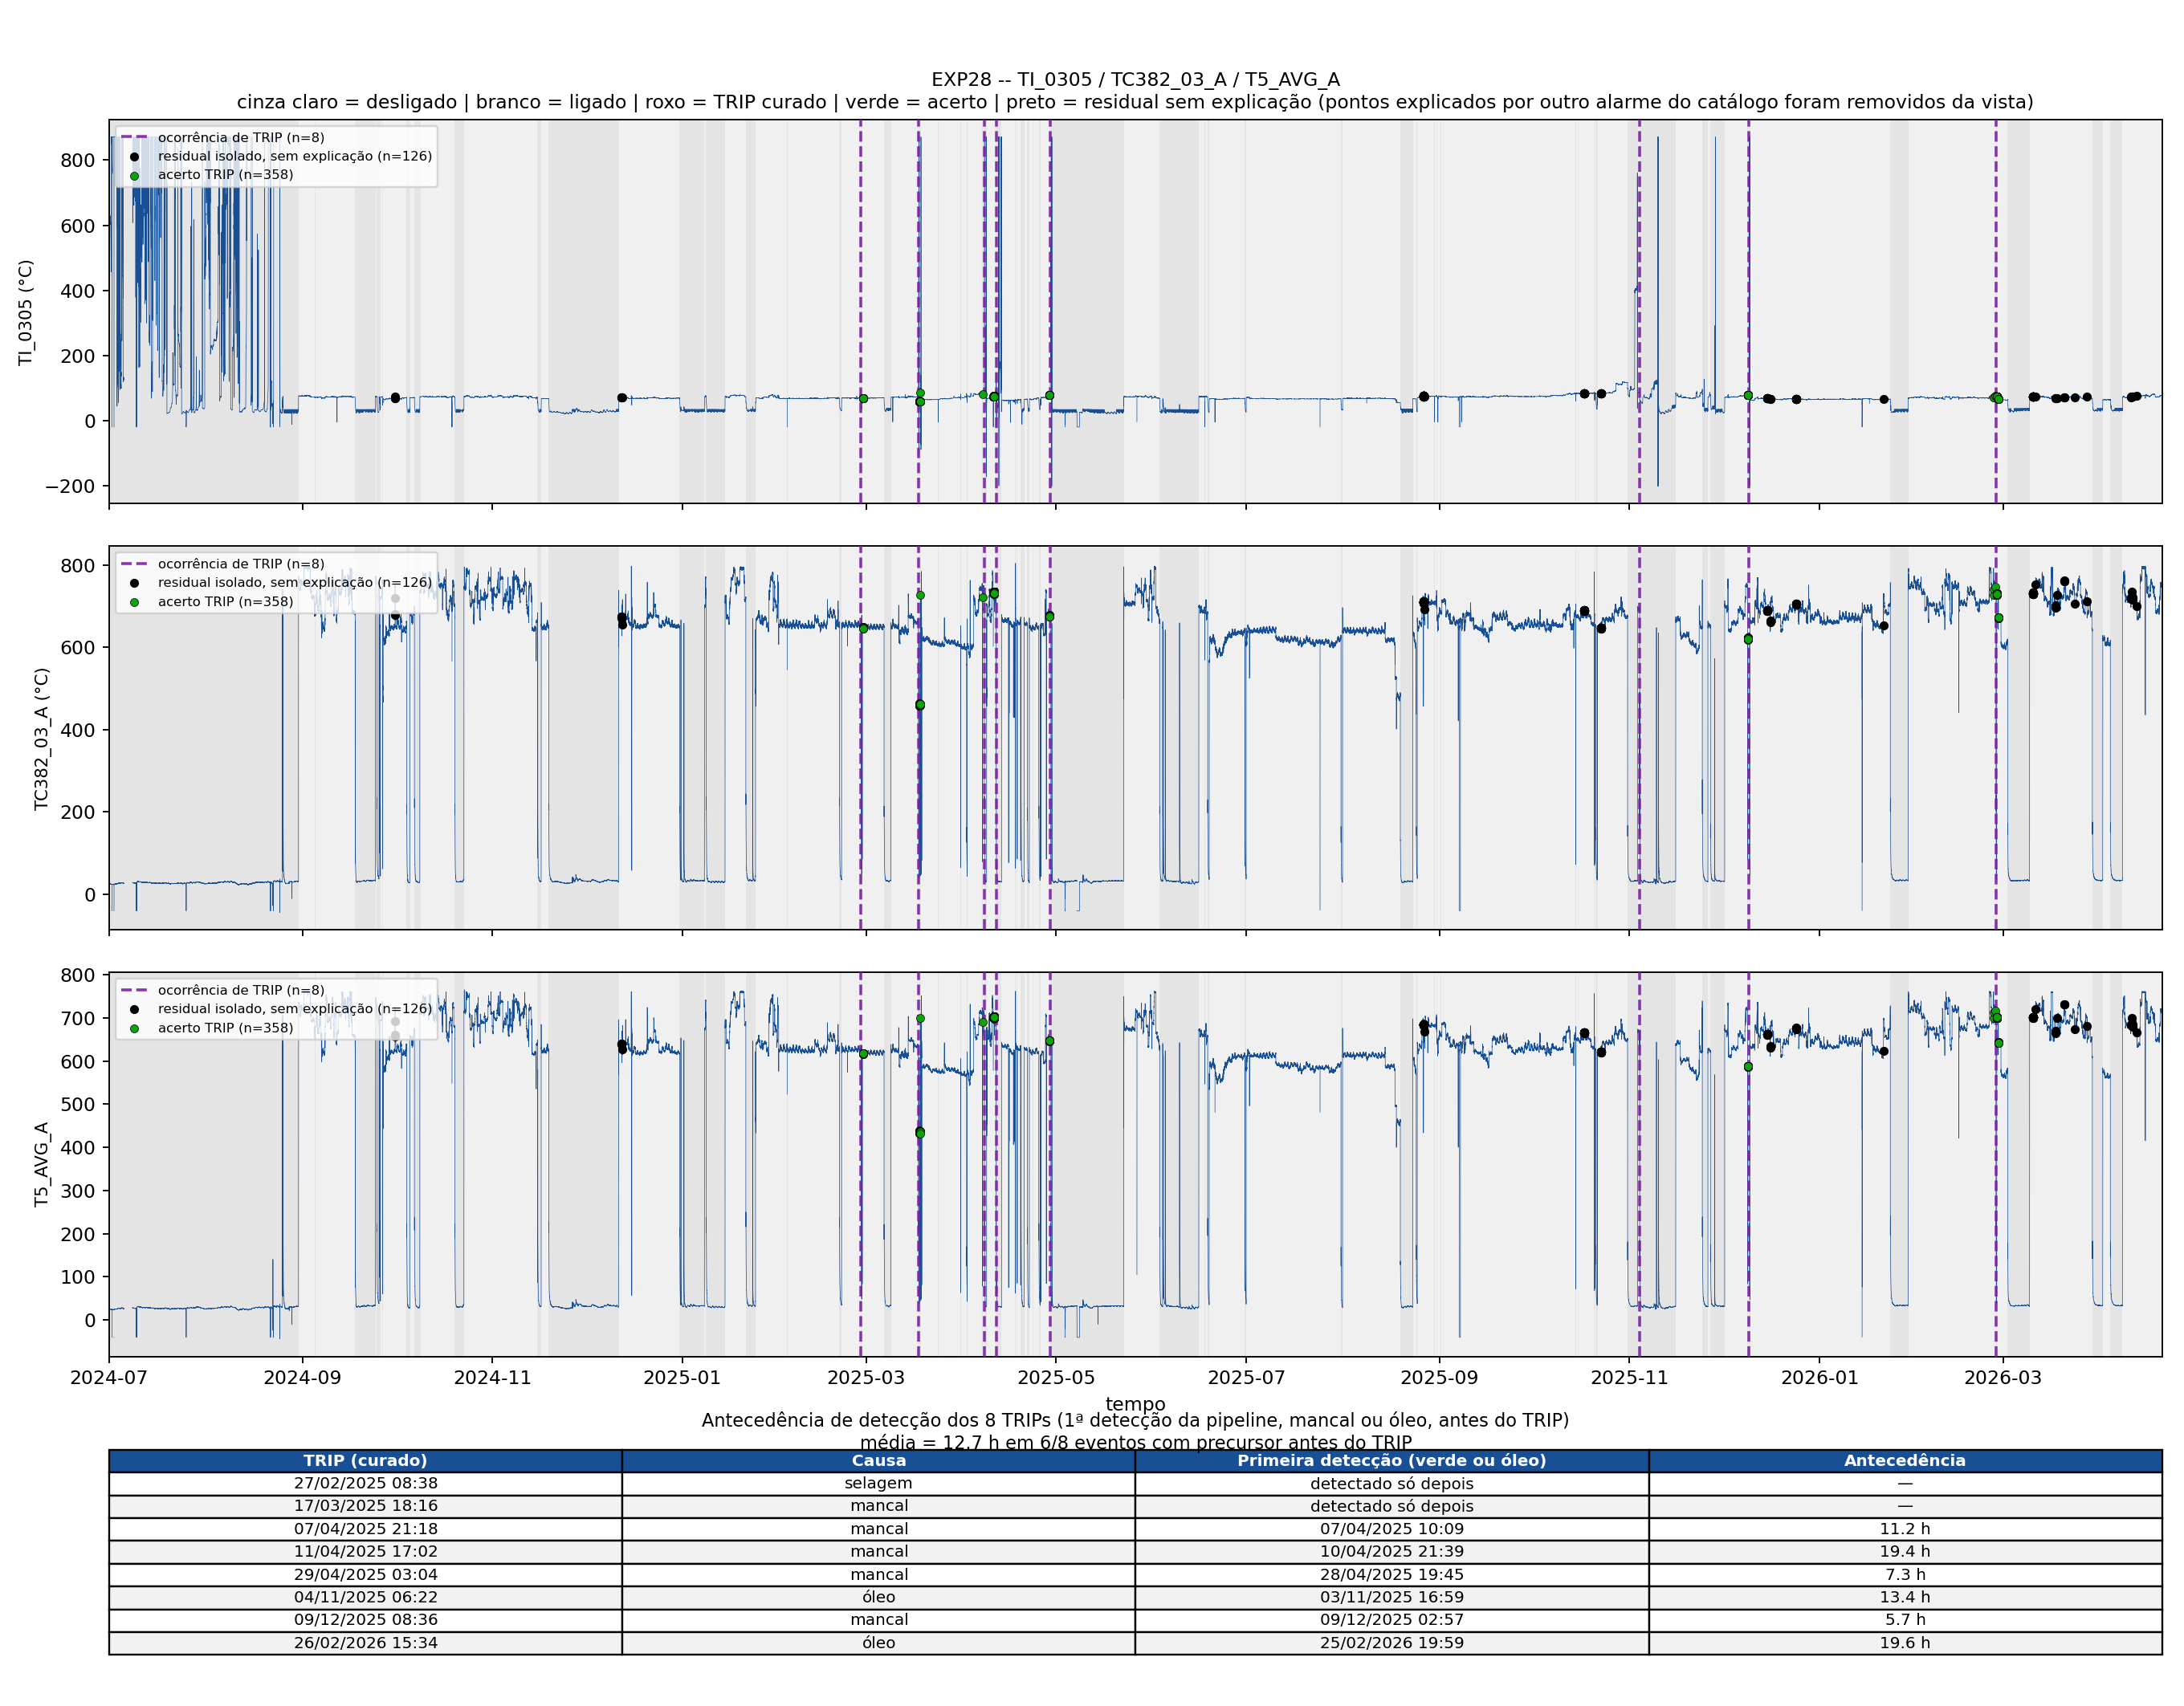
\includegraphics[width=\textwidth]{serie_ti0305_tc382_t5_exp28_v3.png}
\caption{\label{fig:depois}Classificação mascarada (``depois''): fundo
branco = ligado, cinza claro = desligado; linha vertical
\textcolor{corRoxo}{roxa} = ocorrência de TRIP curado (8 no período);
pontos \textcolor{corVerde}{verdes} = acerto de TRIP (358); pontos
pretos = residual isolado, sem explicação (126) -- os 4.692 pontos
laranja e as 142 linhas vermelhas da Figura~\ref{fig:antes} foram
retirados da vista (não dos dados). O painel inferior traz a
antecedência de detecção de cada um dos 8 TRIPs.}
\end{figure}

\textbf{A diferença entre as duas figuras é só de foco visual, não de
dado}: a Figura~\ref{fig:antes} responde "o que explica cada ponto
residual?" (útil para auditar o modelo); a Figura~\ref{fig:depois}
responde "estamos pegando os TRIPs, e o que ainda não sabemos
explicar?" (útil para avaliar a métrica-alvo). As duas convivem -- a
primeira embasa os números da Seção~\ref{sec:cruzamento}, a segunda
embasa a antecedência abaixo.

\subsection{Em quanto tempo conseguimos prever os 8 TRIPs}

Para cada TRIP curado, buscamos a \textbf{primeira detecção} (ponto
verde do modelo de mancal, EXP28, \emph{ou} do modelo de óleo, EXP29)
que ocorre \textbf{antes} do TRIP dentro da janela de $\pm$24h --
diferente da Seção~\ref{sec:resultado-oficial} (que só verifica se
existe algum acerto na janela, antes ou depois), aqui o interesse é
estritamente o tempo de antecipação.

\begin{table}[H]
\centering
\begin{tabular}{lccc}
\toprule
\textbf{TRIP (curado)} & \textbf{Causa} & \textbf{1ª detecção antes do TRIP} & \textbf{Antecedência} \\
\midrule
27/02/2025 08:38 & selagem & detectado só depois & --- \\
17/03/2025 18:16 & mancal & detectado só depois & --- \\
07/04/2025 21:18 & mancal & 07/04/2025 10:09 & 11,2\,h \\
11/04/2025 17:02 & mancal & 10/04/2025 21:39 & 19,4\,h \\
29/04/2025 03:04 & mancal & 28/04/2025 19:45 & 7,3\,h \\
04/11/2025 06:22 & óleo & 03/11/2025 16:59 & 13,4\,h \\
09/12/2025 08:36 & mancal & 09/12/2025 02:57 & 5,7\,h \\
26/02/2026 15:34 & óleo & 25/02/2026 19:59 & 19,6\,h \\
\bottomrule
\end{tabular}
\caption{Antecedência média de \textbf{12,7\,h} nos 6 de 8 eventos com
precursor detectado antes do TRIP. Nos outros 2 (27/02/2025 selagem e
17/03/2025 mancal), a pipeline só reagiu dentro da janela de
$\pm$24h \emph{depois} do TRIP -- ainda conta como "acerto" pela
regra de avaliação oficial (Seção~\ref{sec:resultado-oficial}), mas
não seria antecipação útil operacionalmente para esses dois casos
específicos.}
\end{table}

Achado honesto: nem todo "acerto" é antecipação. Dos 8 TRIPs onde o
modelo reagiu dentro da janela oficial, 6 tiveram aviso prévio real
(5,7\,h a 19,6\,h antes) e 2 só foram capturados depois do evento --
um resultado que deve ser comunicado com essa nuance, não simplesmente
como "8/8 antecipados".

% ======================================================================
\section{Régua rigorosa de avaliação: episódios e antecedência real}
\label{sec:regua-rigorosa}

A tabela de antecedência acima já apontava o problema: a avaliação
usada até aqui (janela $\pm$24h simétrica, Seção~\ref{sec:resultado-oficial})
dá crédito de "acerto" tanto pra uma reação antes quanto depois da
falha. Uma régua mais rigorosa, equivalente ao protocolo oficial do
Francisco (falha = parada real, janela de 48h), corrige essa
distorção:

\begin{enumerate}
  \item \textbf{Agrupar alertas em episódios}: um alerta que
    liga/desliga com menos de 2h de intervalo conta como o mesmo
    episódio (funde runs separados por gap $<$2h).
  \item \textbf{Classificar cada episódio em 3 categorias}:
  \begin{itemize}
    \item \textbf{detecção}: o episódio começa até 48h ANTES de uma
      falha catalogada.
    \item \textbf{inconclusivo}: não antecede uma falha catalogada,
      mas a máquina teve uma parada real ($\geq$2h contínuas) até 48h
      DEPOIS do fim do episódio -- pode ser evento físico real não
      catalogado; não conta a favor nem contra.
    \item \textbf{falso\_positivo}: nenhum dos dois.
  \end{itemize}
\end{enumerate}

Implementado em \texttt{scoring.py}
(\texttt{group\_alerts\_into\_episodes}, \texttt{classify\_episodes\_regua},
\texttt{compute\_regua\_metrics}), validado com caso sintético
controlado antes de aplicar aos dados reais, sem regressão na suíte de
testes (\texttt{15 passed}). Aplicado sobre os
\texttt{point\_anomalies\_all.csv} já calculados do EXP30/31 -- sem
re-treinar nada, só reavalia o mesmo \texttt{is\_anom\_point} com a
régua nova.

\subsection{Resultado: 6 de 8, não 8/8}

\begin{table}[H]
\centering
\begin{tabular}{lccc}
\toprule
& \textbf{EXP30 mancal} & \textbf{EXP31 óleo} & \textbf{Combinado} \\
\midrule
Episódios (gap$<$2h fundido) & 193 & 38 & -- \\
Detecção (falhas únicas) & 5 & 2 & \textbf{6 de 8} \\
Inconclusivo & 56 & 3 & -- \\
Falso positivo & 127 (5,87/mês) & 33 (1,20/mês) & -- \\
\bottomrule
\end{tabular}
\caption{Sob a régua rigorosa, perdemos 2 falhas: 27/02/2025 (selagem,
reagimos 13,0h depois) e 17/03/2025 (mancal, reagimos 7,5h depois) --
exatamente os 2 casos já identificados como "detectado só depois" na
tabela de antecedência.}
\end{table}

\subsection{Achado de complementaridade com o detector do Francisco}

Comparando nossas 2 falhas perdidas com a tabela oficial dele:

\begin{table}[H]
\centering
\small
\begin{tabular}{lcc}
\toprule
\textbf{Falha} & \textbf{Nós (régua rigorosa)} & \textbf{Francisco (oficial)} \\
\midrule
27/02/2025 selagem & \textcolor{corVermelho}{\ding{55}} (reagiu depois) & \textcolor{corVerde}{\ding{51}} 33,2h \\
17/03/2025 mancal & \textcolor{corVermelho}{\ding{55}} (reagiu depois) & \textcolor{corVerde}{\ding{51}} 30,7h \\
07/04, 11/04, 29/04/2025 mancal & \textcolor{corVerde}{\ding{51}} & \textcolor{corVerde}{\ding{51}} \\
04/11/2025 óleo & \textcolor{corVerde}{\ding{51}} 13,4h & \textcolor{corVermelho}{\ding{55}} (limitação de observabilidade) \\
09/12/2025 mancal & \textcolor{corVerde}{\ding{51}} 5,7h & \textcolor{corVermelho}{\ding{55}} (varreu 36 sensores, nada achou) \\
26/02/2026 óleo & \textcolor{corVerde}{\ding{51}} (bônus, via mancal) & \textcolor{corVerde}{\ding{51}} 19,9h \\
\bottomrule
\end{tabular}
\end{table}

\textbf{Somos 6/8, ele é 6/8 -- empatados, não superiores.} Mas em
conjuntos diferentes: nossos 2 misses são exatamente os 2 acertos
dele, e nossos 2 acertos exclusivos (04/11 óleo, 09/12 mancal) são
exatamente os 2 casos que ele documenta como falha do próprio sistema.
\textbf{Combinando as duas abordagens, dá 8/8} -- evidência de
complementaridade real entre as duas arquiteturas de detecção (a
nossa multiescala/AutoML e a PCA de 4 sinais dele), não de que uma
supera a outra. Argumento a favor de operar os dois sistemas em
paralelo, não de substituir um pelo outro.

% ======================================================================
\section{Conclusão e próximos passos}
\label{sec:conclusao}

A pipeline de produção (EXP28/29) mantém 100\% da detecção já validada
(90\% no catálogo de 40 alarmes, 100\% nos 2 TRIPs de óleo), com uma
proteção extra sem custo (veto de sensor congelado). Contra o
ground-truth curado do Francisco, sob a régua rigorosa
(Seção~\ref{sec:regua-rigorosa}) o resultado correto é \textbf{6 de 8}
com antecedência real -- empatado com o detector oficial dele, com um
achado de complementaridade (nossos 2 misses são exatamente os 2
acertos dele, e vice-versa) mais valioso que um número inflado de
8/8. O que parecia FP residual, quando
investigado com a mesma disciplina de reconstrução literal usada em
toda a sessão, revelou-se \textbf{88,1\% sinal real não reconhecido} --
e dos 11,9\% restantes, mais de 90\% também se explicam por padrão
físico recorrente ou artefato estrutural inevitável de portões causais.

\textbf{Próximo passo}: implementar uma \textbf{supressão cirúrgica
baseada em mecanismo} para a Categoria~2 (borda de portão causal) --
diferente do 2º filtro de duração genérico já testado e rejeitado
(Seção~\ref{sec:fechamento24}), essa supressão só atua quando o
critério causal específico (portão engatando logo em seguida) é
verificado, não por duração isolada. Implementação e validação em
andamento, registradas em
\texttt{docs/analise\_automl\_exp10.md}.

\subsection*{Referência: por que o 2º filtro de duração genérico falhou}
\label{sec:2ofiltro}
Testado anteriormente (aplicar um filtro de duração mínima
\emph{depois} de todos os portões, não antes): manteve 100\% de
detecção só no limiar mais suave (1\,min), mas já custava 3 alarmes
reais logo ali; em limiares maiores o hit\_rate caía a 37,5\% sem
reduzir o FP de forma proporcional. Causa raiz: nesse ponto da cadeia,
um fragmento curto de precursor real truncado por um portão e um
fragmento curto de ruído genuíno são \textbf{indistinguíveis por
duração} -- por isso a supressão cirúrgica precisa usar o critério
causal (portão real engatando), não duração isolada.

% ======================================================================
\section{Por que dois experimentos separados (mancal e óleo)?}
\label{sec:porque-dois-experimentos}

A pipeline roda como \textbf{dois experimentos independentes}, cada um
com seu próprio grupo de sensores, seu próprio modelo e sua própria
config JSON:

\begin{table}[H]
\centering
\small
\begin{tabular}{p{3cm}p{5.7cm}p{5.7cm}}
\toprule
& \textbf{EXP28/30 -- mancal} & \textbf{EXP29/31 -- óleo} \\
\midrule
Sensores-alvo & TC382\_03\_A, T5\_AVG\_A (temperatura de mancal) & PI\_0308 (pressão de óleo), PDIT\_0305 (diferencial de selagem) \\
Sensores de contexto & 10 canais de vibração (\texttt{TV\_*}) & os mesmos 10 canais de vibração \\
Modelo & OCSVM & Isolation Forest \\
Mecanismo de falha & desgaste/aquecimento de mancal & perda de pressão/vazamento de óleo lubrificante \\
\bottomrule
\end{tabular}
\end{table}

\textbf{Isso não é uma limitação técnica -- é uma escolha de
arquitetura validada empiricamente duas vezes nesta investigação:}

\begin{enumerate}
  \item \textbf{Mancal e óleo são mecanismos físicos distintos}, com
    sensores-alvo diferentes e dinâmicas diferentes (temperatura de
    mancal evolui em horas; pressão de óleo pode cair em minutos). Um
    único modelo treinado sobre os 4 sensores-alvo ao mesmo tempo tem
    que aprender uma noção de "normal" que mistura os dois regimes --
    dilui a sensibilidade do modelo para o mecanismo mais sutil de
    cada evento.
  \item \textbf{Testamos exatamente essa unificação (EXP27,
    Seção~\ref{sec:unificado}) e ela piorou}: 7 de 9 contra os 8 de 8
    obtidos com os dois modelos especializados juntos. Os 2 eventos
    perdidos foram justamente os mais sutis de cada mecanismo --
    exatamente onde a diluição por sensores irrelevantes do outro
    subsistema pesa mais.
  \item \textbf{É a mesma lição que já orienta o detector de produção
    do Francisco}: ele usa 4 sinais independentes (temperatura,
    pressão de óleo, \textit{spread} de mancal, selagem) em vez de um
    modelo único sobre os 39 sensores -- chegamos à mesma conclusão de
    forma independente.
\end{enumerate}

Na prática, os dois experimentos rodam em paralelo e alimentam o mesmo
dashboard -- o operador não precisa saber que são dois modelos
por trás; ele só recebe alertas de mancal e de óleo, cada um calibrado
especificamente pro seu próprio mecanismo de falha.

% ======================================================================
\section{Como isso funciona operacionalmente}
\label{sec:operacional}

A anotação de contexto (\texttt{ENABLE\_ALERT\_CATALOG\_CONTEXT},
implementada nos experimentos EXP30/31) roda como o \textbf{último
passo} da pipeline, depois de todos os portões já terem decidido
\texttt{is\_anom\_point} -- ela nunca decide, apenas acrescenta
contexto (\texttt{alert\_catalog\_tag}, \texttt{alert\_catalog\_time},
\texttt{alert\_catalog\_distance\_h}, \texttt{alert\_confidence}) para
quem consome o alerta.

\subsection{O que é removido de verdade, e o que só é ocultado/anotado}
\label{sec:tratamento-fp-final}

Vale deixar explícita a distinção entre 3 coisas que podem parecer
iguais mas não são:

\begin{enumerate}
  \item \textbf{Removido de verdade, dentro da modelagem}: os portões
    (rampa de carga, volatilidade, mudança de nível, veto de sensor
    congelado, filtro de duração mínima) suprimem \texttt{is\_anom\_point}
    de fato, como parte da pipeline de produção (EXP28/29/30/31). É
    seguro e validado -- remove ruído estrutural sem custar detecção
    real.
  \item \textbf{Não removido dos dados -- só ocultado da Figura~\ref{fig:depois}}:
    os pontos laranja (explicados por outro alarme do catálogo, não
    TRIP). Eles continuam em \texttt{point\_anomalies\_all.csv} como
    \texttt{is\_anom\_point=1}; só saem do desenho porque, para a
    pergunta "detectamos os TRIPs?", eles não agregam mais informação
    (Seção~\ref{sec:figura-depois}).
  \item \textbf{Proposto para remover de verdade e REJEITADO}: a
    supressão cirúrgica baseada em mecanismo (Seção~\ref{sec:fechamento24})
    -- suprimiria pontos isolados seguidos de um portão engatando, mas
    isso também mataria 3 precursores reais de TRIP (07/04/2025 e
    26/02/2026), porque um precursor real truncado por um portão e
    ruído genuíno têm a mesma assinatura. Nenhum código de produção
    foi alterado para implementar essa remoção.
\end{enumerate}

\begin{figure}[H]
\centering
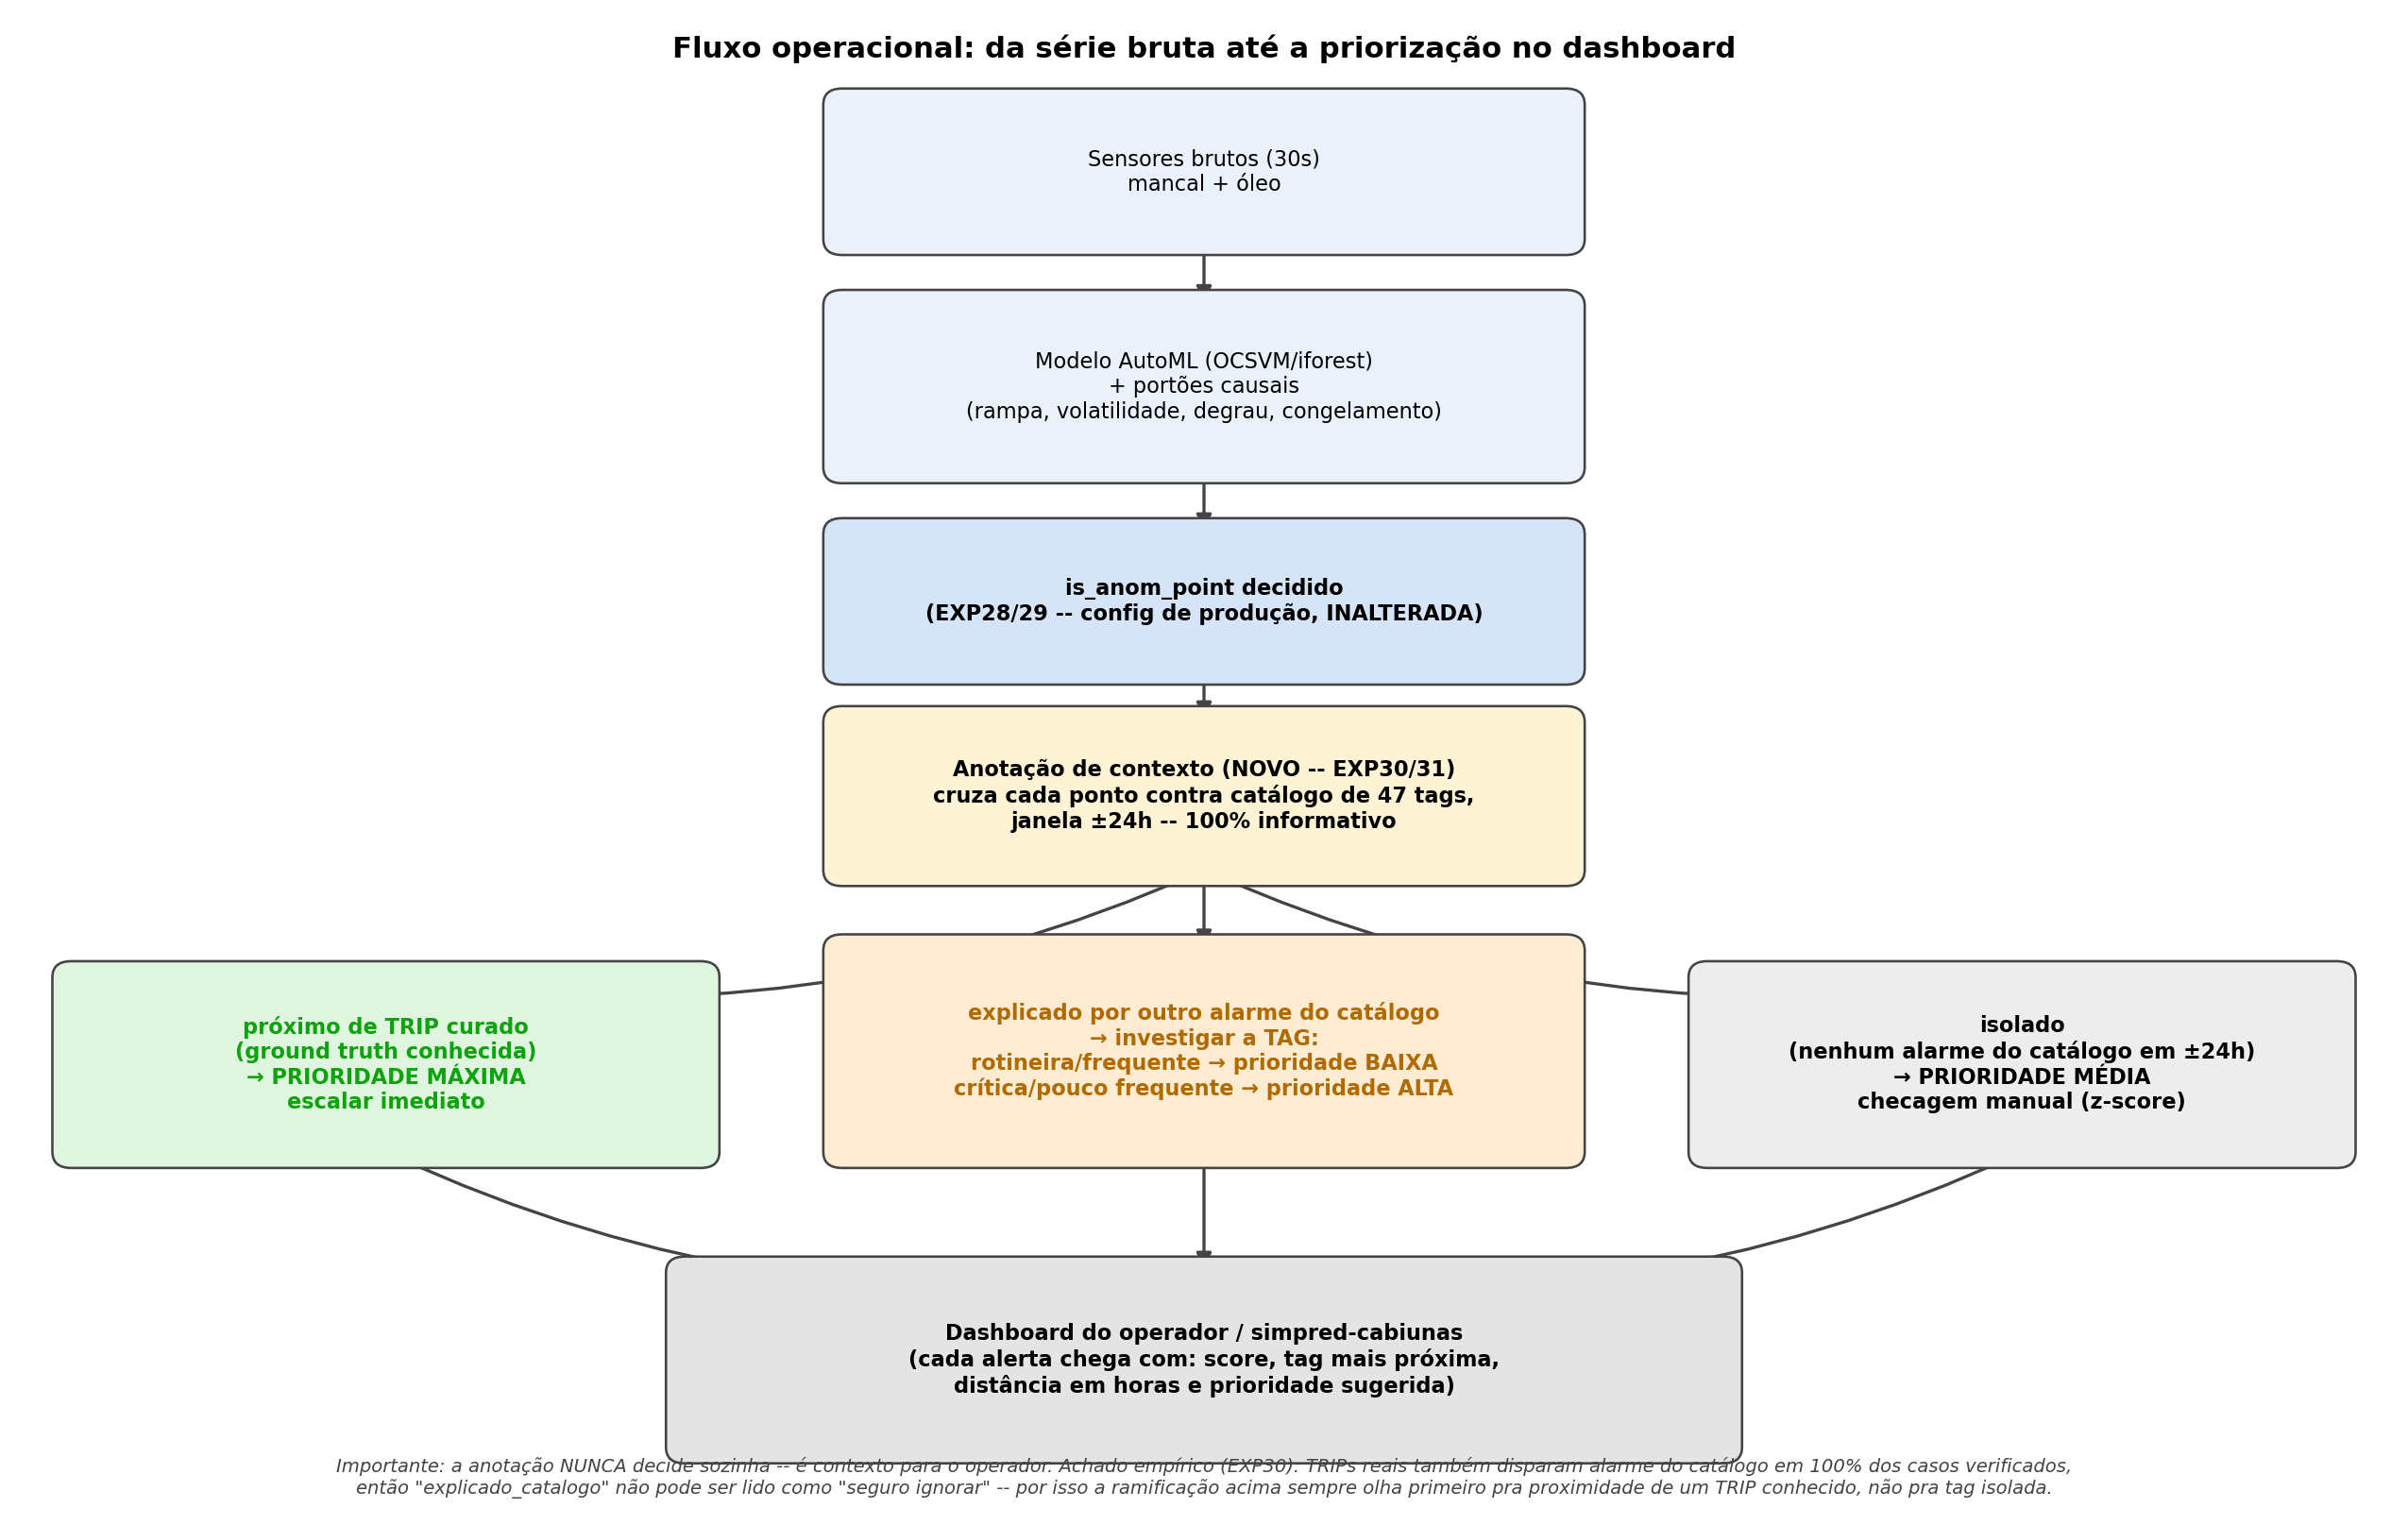
\includegraphics[width=0.92\textwidth]{diagrama_fluxo_operacional.png}
\caption{Fluxo operacional completo: da série bruta até a priorização
sugerida no dashboard. A anotação de contexto (caixa amarela) é
puramente aditiva -- \texttt{is\_anom\_point} já está decidido antes
dela.}
\end{figure}

\subsection{Achado importante: TRIP real também dispara o catálogo}

Antes de sugerir qualquer regra de priorização, verificamos se os 358
pontos verdes (acerto de TRIP) também apareciam marcados como
\texttt{explicado\_catalogo}. Resultado:

\begin{table}[H]
\centering
\begin{tabular}{lcc}
\toprule
& \textbf{explicado\_catalogo} & \textbf{isolado} \\
\midrule
Perto de TRIP curado (358 pontos) & \textbf{358 (100\%)} & 0 \\
Longe de TRIP curado (4.818 pontos) & 4.692 (97,4\%) & 126 (2,6\%) \\
\bottomrule
\end{tabular}
\caption{Todo TRIP real do período também disparou algum alarme do
catálogo de 47 tags dentro de $\pm$24h -- faz sentido fisicamente,
uma falha real de mancal ou óleo tende a disparar vários alarmes de
processo ao mesmo tempo, não só o nosso modelo.}
\end{table}

\textbf{Consequência prática: a tag \texttt{alert\_confidence =
"explicado\_catalogo"} sozinha NÃO pode ser lida como "seguro
ignorar"} -- ela só diz que existe outro alarme por perto, não diz se
é o mesmo evento real (como um TRIP) ou um alarme de processo
rotineiro sem relação. Por isso a árvore de decisão do diagrama acima
sempre checa primeiro a proximidade de um TRIP conhecido; só depois
disso é que a tag específica do catálogo (rotineira vs. crítica) entra
como critério de priorização.

\subsection{Três casos reais, lado a lado}

\begin{figure}[H]
\centering
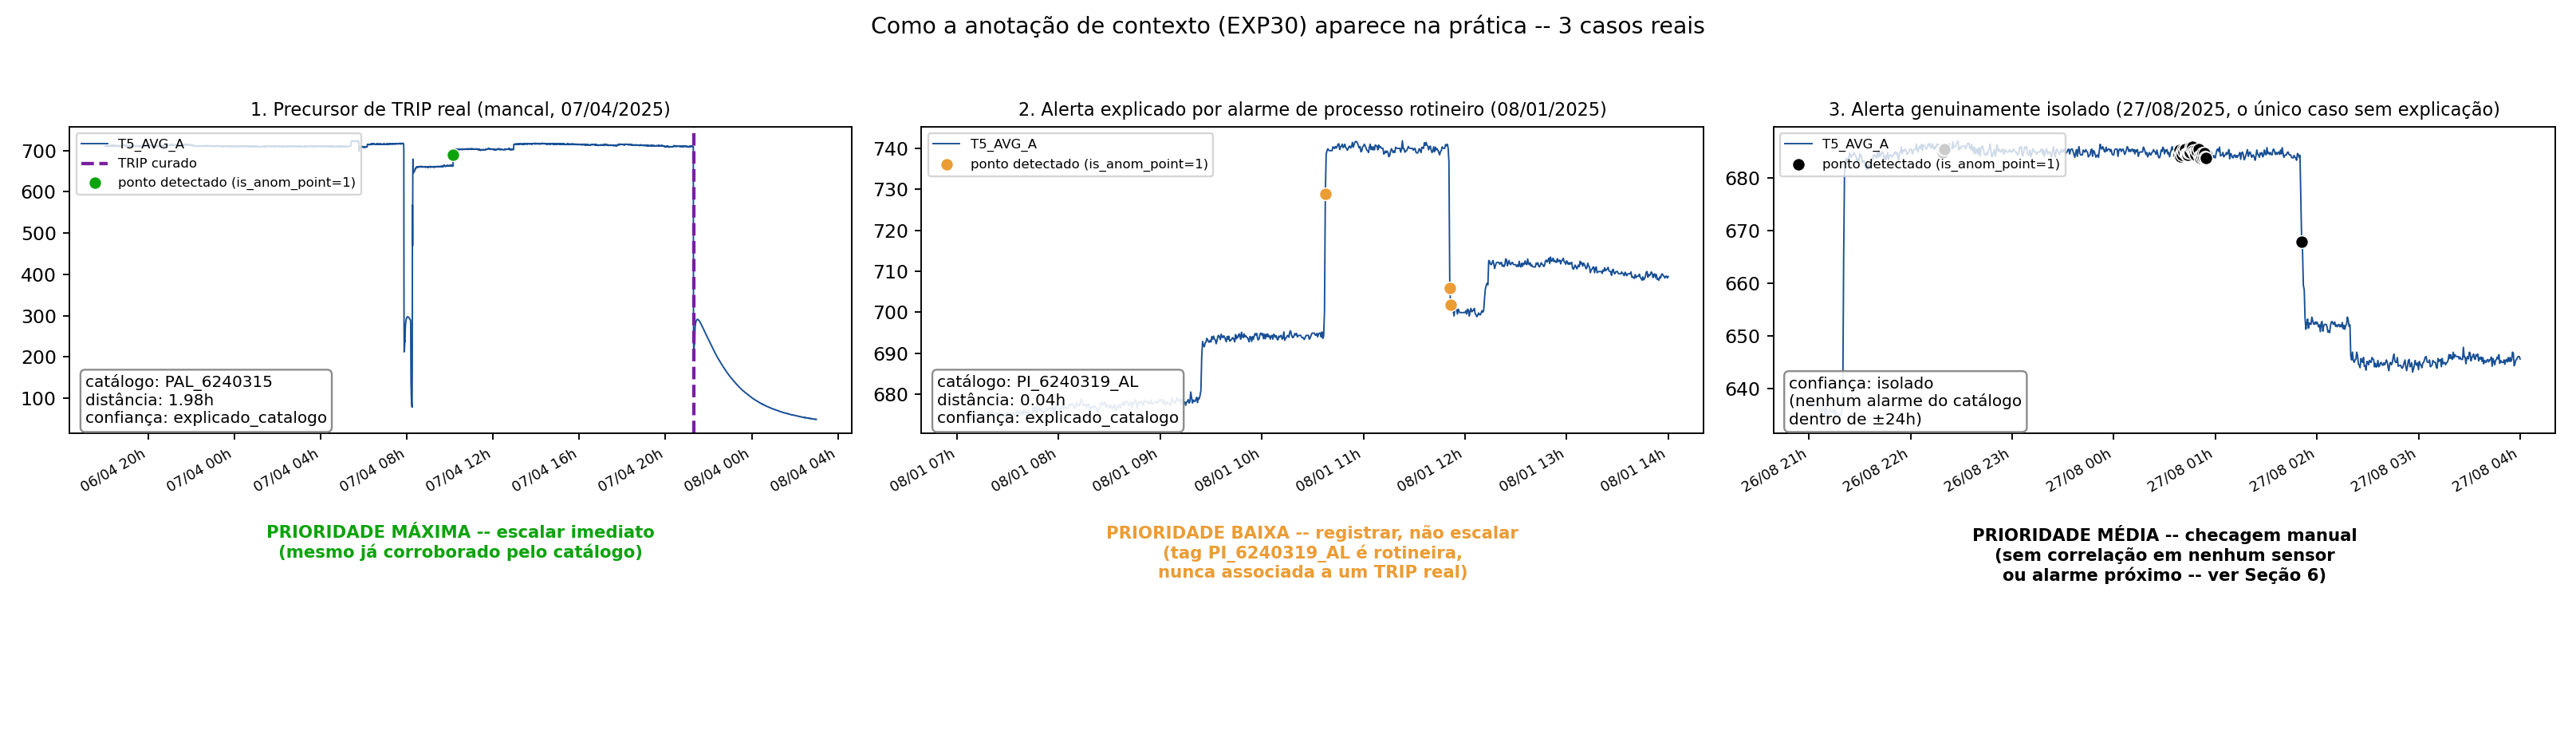
\includegraphics[width=\textwidth]{figura_operacional_exemplos.png}
\caption{Três alertas reais e como o dashboard os apresentaria. (1) Um
precursor real de TRIP (07/04/2025) -- prioridade máxima, mesmo já
corroborado pelo catálogo (\texttt{PAL\_6240315}, 1,98\,h de
distância). (2) Um alerta explicado por uma tag rotineira
(\texttt{PI\_6240319\_AL}, a mais frequente do catálogo, nunca
associada a um TRIP real) -- prioridade baixa. (3) O único alerta
genuinamente isolado de toda a investigação (27/08/2025) -- prioridade
média, mesmo status do caso descrito na Seção~\ref{sec:fechamento24}.}
\end{figure}

\subsection{Resumo da regra de priorização sugerida}

\begin{table}[H]
\centering
\small
\begin{tabular}{p{4.3cm}p{4.3cm}p{5.4cm}}
\toprule
\textbf{Situação} & \textbf{Prioridade} & \textbf{Ação sugerida} \\
\midrule
Perto de um TRIP/falha curada conhecida & Máxima & Escalar imediatamente, independente de qualquer outra tag \\
Explicado por tag do catálogo pouco frequente/crítica & Alta & Investigar -- pode ser o mesmo evento real disparando dois alarmes \\
Explicado por tag do catálogo rotineira/muito frequente (ex: \texttt{PI\_6240319\_AL}) & Baixa & Registrar, não escalar automaticamente \\
Isolado (nenhum alarme do catálogo em $\pm$24h) & Média & Checagem manual (mesma disciplina de z-score da Seção~\ref{sec:fechamento24}) -- historicamente metade desses casos eram sinal físico real \\
\bottomrule
\end{tabular}
\caption{Nenhuma dessas linhas suprime um alerta -- todas continuam
aparecendo no dashboard, só mudam a ordem/urgência de atenção do
operador.}
\end{table}

\end{document}
